\documentclass[10pt, conference]{IEEEtran}
\usepackage[spanish]{babel} 
\usepackage[utf8]{inputenc}
\usepackage{amsmath}
\usepackage{graphicx}
\usepackage[colorinlistoftodos]{todonotes}
\usepackage{fancyhdr}
\usepackage{cite}
\pagestyle{fancy}
\fancyhf{} 
\fancyhead[LO]{\leftmark} 
\fancyhead[RE]{\rightmark} 
\fancyhead[RO,LE]{\thepage} 
\fancyfoot[LE,RO]{Criptografía Asimétrica}   
\renewcommand{\footrulewidth}{0.3pt}
\title{Criptografía Asimétrica}

\begin{document}
\maketitle

\section{Conceptos Básicos}

La criptografía Asimétrica, conocida también como criptografía de dos claves o criptografía de clave pública, es aquella en la cual el método criptográfico utilizado consta de un par de claves que serán usadas en el tratamiento de los mensajes. Dichas claves pertenecen al autor del mensaje siendo la de tipo pública, aquella que se puede entregar a cualquier otra persona, mientras que la otra de tipo "privada" será de uso exclusivo para el dueño, quién deberá evitar, bajo cualquier circunstancia, compartirla.

El funcionamiento de este metodo va de la siguiente manera:
\begin{itemize}
\item El remitente usa la clave pública del destinatario para cifrar el mensaje.
\item Usando la clave privada, el destinatario podrá descifrar el mensaje.

\item De la misma manera, el propietario podrá cifrar mensajes para que aquellos que dispongan de la clave pública puedan descifrarlo.

\item De esta manera se garantiza la confindencialidad del mensaje ya que nadie, salvo el destinatario, puede descifrarlo.

\end{itemize}

\begin{figure}[h]
\begin{center}
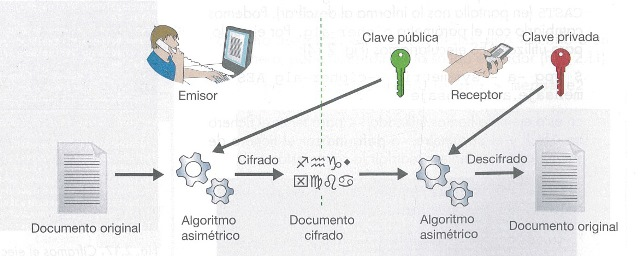
\includegraphics[scale=0.60]{asimetrica.jpg} \end{center}
\caption{Esquema de la Criptografía Asimétrica}
\end{figure}

\subsection{Ventajas de la Criptografía Asimetrica}
\begin{itemize}
\item Una las ventajas mas resaltantes es  la facilidad y seguridad con la que las llaves publicas se pueden distribuir.
\item No existe el desbordamiento en el tratamiento de claves y canales.
\item Otra ventaja en menor medida, es que a pesar de que en el trasfondo de la Criptografía Asimetrica exista un algoritmo capaz de generar claves, es casi imposible que dos personas obtengan la misma pareja de claves.
\end{itemize}

\subsection{Desventajas de la Criptografía Asimétrica}
\begin{itemize}
\item Para generar una clave de la misma longitud se necesita mayor tiempo de proceso.(Supone un problema de lentitud)
\item Es muy probable que este sistema falle si las claves son muchos menores que las simetricas.
\item El mensaje cifrado ocupa un espacio mayor al mensaje original.
\item Generalmente el uso continuo de las claves privadas conlleva a recibir ataque criptográficos con sistemas capaces de analizar paquetes cifrados (Caso Sony diciembre 2010).
\item Es necesario proteger la clave privada. Generalmente esto se hace almacenando todas las llaves privadas dentro de un archivo privado "llavero" que estará protegido con cifrado simétrico.
\item Hay que transportar la claves privadas, suponieno el riesgo mismo de extraviar el llavero 
\end{itemize}

\section{Diffie-Hellman}
El protocolo de cifrado Diffie-Hellman (recibe el nombre de sus creadores) es un sistema de intercambio de claves entre partes, que no han contactado previamente, a través de un canal inseguro y sin autenticación.
Este protocolo se utiliza principalmente para intercambiar claves simétricas de forma segura para posteriormente pasar a utilizar un cifrado simétrico, menos costoso que el asimétrico.
Se parte de la idea de que dos interlocutores pueden generar de forma conjunta una clave sin que esta sea comprometida.
\subsection{Funcionamiento}
\begin{enumerate}
\item Se escoge un número primo $p$ y un generador $g$, siendo este último coprimo de $p$. Ambos números son públicos.
\item Escogemos un número a menor que $p$, en este caso $a$, y calculamos:
\medskip
\[
A = g^a  mod p 
\]
\medskip
Enviamos $A$, $p$ y $g$ al otro interlocutor.
\item El otro interlocutor escoge un numero $b$ menor que $p$ y calcula:
\medskip
\[
B = g^b mod p
\]
\medskip
Retornandonos $B$.
\item Ahora, ambos podemos calcular:
\medskip
\[
K = g^(a-b)mod p
\]
\medskip
Siendo para nosotros $B^a mod p = K$ y para nuestro interlocutor $A^b mod p = K$. Usamos $K$ como clave.
\item Al ser $p$ y $g$ públicos cualquier atacante puede llegar a conocerlos, esto no supone una vulnerabilidad. Aunque capturase $A$ y $B$, le resultaría computacionalmente imposible obtener $a$ y $b$ con la consecuencia de tampoco acceder a $K$. 
\end{enumerate}

\begin{figure}[h]
\begin{center}
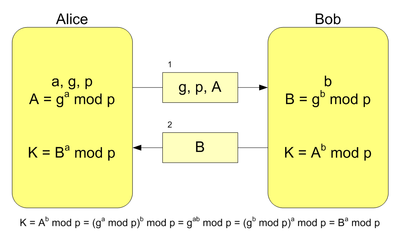
\includegraphics[scale=0.60]{Diffie.png} \end{center}
\caption{Funcionamiento del sistema Diffie-Hellman}
\end{figure}

\subsection{Vulnerabilidades}
Este protocolo es vulnerable al ataque "man in the middle"; el cual consiste en que un tercero se coloca en el medio del canal y hace creer a ambos que es el otro. De esta forma se podría acordar una clave con cada parte y servir de "enlace" entre los dos participantes. Para que este ataque sea funcional se necesita saber que método de cifrado simétrico se va a emplear. Ocultar el algoritmo de cifrado no cumple con el principio de Kerkckhoffs de que la efectividad de un sistema no debe depender de que su diseño
permanezca en secreto por lo que conocer el sistema que se va a emplear se hace trivial.

Para evitar esto se puede emplear un protocolo de autenticación de las partes mediante por ejemplo TLS(Transport Layer Security).

\begin{figure}[h]
\begin{center}
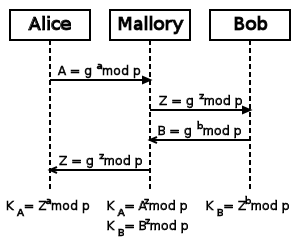
\includegraphics[scale=0.60]{man.png} \end{center}
\caption{Esquema de la intrusión Man-in-the-middle}
\end{figure}




\bibliographystyle{plain}
\bibliography{biblio.bib}

\end{document}

 
 


